\documentclass[1p]{elsarticle_modified}
%\bibliographystyle{elsarticle-num}

%\usepackage[colorlinks]{hyperref}
%\usepackage{abbrmath_seonhwa} %\Abb, \Ascr, \Acal ,\Abf, \Afrak
\usepackage{amsfonts}
\usepackage{amssymb}
\usepackage{amsmath}
\usepackage{amsthm}
\usepackage{scalefnt}
\usepackage{amsbsy}
\usepackage{kotex}
\usepackage{caption}
\usepackage{subfig}
\usepackage{color}
\usepackage{graphicx}
\usepackage{xcolor} %% white, black, red, green, blue, cyan, magenta, yellow
\usepackage{float}
\usepackage{setspace}
\usepackage{hyperref}

\usepackage{tikz}
\usetikzlibrary{arrows}

\usepackage{multirow}
\usepackage{array} % fixed length table
\usepackage{hhline}

%%%%%%%%%%%%%%%%%%%%%
\makeatletter
\renewcommand*\env@matrix[1][\arraystretch]{%
	\edef\arraystretch{#1}%
	\hskip -\arraycolsep
	\let\@ifnextchar\new@ifnextchar
	\array{*\c@MaxMatrixCols c}}
\makeatother %https://tex.stackexchange.com/questions/14071/how-can-i-increase-the-line-spacing-in-a-matrix
%%%%%%%%%%%%%%%

\usepackage[normalem]{ulem}

\newcommand{\msout}[1]{\ifmmode\text{\sout{\ensuremath{#1}}}\else\sout{#1}\fi}
%SOURCE: \msout is \stkout macro in https://tex.stackexchange.com/questions/20609/strikeout-in-math-mode

\newcommand{\cancel}[1]{
	\ifmmode
	{\color{red}\msout{#1}}
	\else
	{\color{red}\sout{#1}}
	\fi
}

\newcommand{\add}[1]{
	{\color{blue}\uwave{#1}}
}

\newcommand{\replace}[2]{
	\ifmmode
	{\color{red}\msout{#1}}{\color{blue}\uwave{#2}}
	\else
	{\color{red}\sout{#1}}{\color{blue}\uwave{#2}}
	\fi
}

\newcommand{\Sol}{\mathcal{S}} %segment
\newcommand{\D}{D} %diagram
\newcommand{\A}{\mathcal{A}} %arc


%%%%%%%%%%%%%%%%%%%%%%%%%%%%%5 test

\def\sl{\operatorname{\textup{SL}}(2,\Cbb)}
\def\psl{\operatorname{\textup{PSL}}(2,\Cbb)}
\def\quan{\mkern 1mu \triangleright \mkern 1mu}

\theoremstyle{definition}
\newtheorem{thm}{Theorem}[section]
\newtheorem{prop}[thm]{Proposition}
\newtheorem{lem}[thm]{Lemma}
\newtheorem{ques}[thm]{Question}
\newtheorem{cor}[thm]{Corollary}
\newtheorem{defn}[thm]{Definition}
\newtheorem{exam}[thm]{Example}
\newtheorem{rmk}[thm]{Remark}
\newtheorem{alg}[thm]{Algorithm}

\newcommand{\I}{\sqrt{-1}}
\begin{document}

%\begin{frontmatter}
%
%\title{Boundary parabolic representations of knots up to 8 crossings}
%
%%% Group authors per affiliation:
%\author{Yunhi Cho} 
%\address{Department of Mathematics, University of Seoul, Seoul, Korea}
%\ead{yhcho@uos.ac.kr}
%
%
%\author{Seonhwa Kim} %\fnref{s_kim}}
%\address{Center for Geometry and Physics, Institute for Basic Science, Pohang, 37673, Korea}
%\ead{ryeona17@ibs.re.kr}
%
%\author{Hyuk Kim}
%\address{Department of Mathematical Sciences, Seoul National University, Seoul 08826, Korea}
%\ead{hyukkim@snu.ac.kr}
%
%\author{Seokbeom Yoon}
%\address{Department of Mathematical Sciences, Seoul National University, Seoul, 08826,  Korea}
%\ead{sbyoon15@snu.ac.kr}
%
%\begin{abstract}
%We find all boundary parabolic representation of knots up to 8 crossings.
%
%\end{abstract}
%\begin{keyword}
%    \MSC[2010] 57M25 
%\end{keyword}
%
%\end{frontmatter}

%\linenumbers
%\tableofcontents
%
\newcommand\colored[1]{\textcolor{white}{\rule[-0.35ex]{0.8em}{1.4ex}}\kern-0.8em\color{red} #1}%
%\newcommand\colored[1]{\textcolor{white}{ #1}\kern-2.17ex	\textcolor{white}{ #1}\kern-1.81ex	\textcolor{white}{ #1}\kern-2.15ex\color{red}#1	}

{\Large $\underline{11a_{264}~(K11a_{264})}$}

\setlength{\tabcolsep}{10pt}
\renewcommand{\arraystretch}{1.6}
\vspace{1cm}\begin{tabular}{m{100pt}>{\centering\arraybackslash}m{274pt}}
\multirow{5}{120pt}{
	\centering
	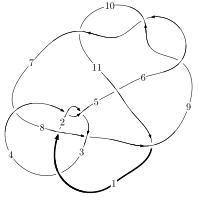
\includegraphics[width=112pt]{../../../GIT/diagram.site/Diagrams/png/513_11a_264.png}\\
\ \ \ A knot diagram\footnotemark}&
\allowdisplaybreaks
\textbf{Linearized knot diagam} \\
\cline{2-2}
 &
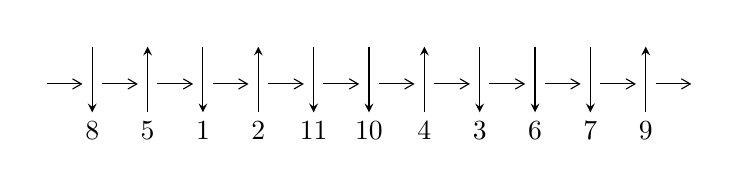
\begin{tikzpicture}[x=20pt, y=17pt]
	% nodes
	\node (C0) at (0, 0) {};
	\node (C1) at (1, 0) {};
	\node (C1U) at (1, +1) {};
	\node (C1D) at (1, -1) {8};

	\node (C2) at (2, 0) {};
	\node (C2U) at (2, +1) {};
	\node (C2D) at (2, -1) {5};

	\node (C3) at (3, 0) {};
	\node (C3U) at (3, +1) {};
	\node (C3D) at (3, -1) {1};

	\node (C4) at (4, 0) {};
	\node (C4U) at (4, +1) {};
	\node (C4D) at (4, -1) {2};

	\node (C5) at (5, 0) {};
	\node (C5U) at (5, +1) {};
	\node (C5D) at (5, -1) {11};

	\node (C6) at (6, 0) {};
	\node (C6U) at (6, +1) {};
	\node (C6D) at (6, -1) {10};

	\node (C7) at (7, 0) {};
	\node (C7U) at (7, +1) {};
	\node (C7D) at (7, -1) {4};

	\node (C8) at (8, 0) {};
	\node (C8U) at (8, +1) {};
	\node (C8D) at (8, -1) {3};

	\node (C9) at (9, 0) {};
	\node (C9U) at (9, +1) {};
	\node (C9D) at (9, -1) {6};

	\node (C10) at (10, 0) {};
	\node (C10U) at (10, +1) {};
	\node (C10D) at (10, -1) {7};

	\node (C11) at (11, 0) {};
	\node (C11U) at (11, +1) {};
	\node (C11D) at (11, -1) {9};
	\node (C12) at (12, 0) {};

	% arrows
	\draw[->,>={angle 60}]
	(C0) edge (C1) (C1) edge (C2) (C2) edge (C3) (C3) edge (C4) (C4) edge (C5) (C5) edge (C6) (C6) edge (C7) (C7) edge (C8) (C8) edge (C9) (C9) edge (C10) (C10) edge (C11) (C11) edge (C12) ;	\draw[->,>=stealth]
	(C1U) edge (C1D) (C2D) edge (C2U) (C3U) edge (C3D) (C4D) edge (C4U) (C5U) edge (C5D) (C6U) edge (C6D) (C7D) edge (C7U) (C8U) edge (C8D) (C9U) edge (C9D) (C10U) edge (C10D) (C11D) edge (C11U) ;
	\end{tikzpicture} \\
\hhline{~~} \\& 
\textbf{Solving Sequence} \\ \cline{2-2} 
 &
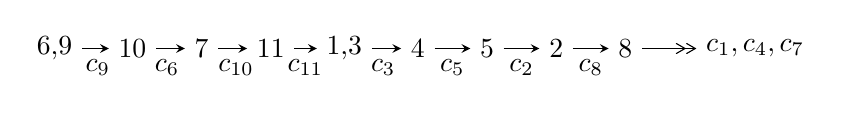
\begin{tikzpicture}[x=25pt, y=7pt]
	% node
	\node (A0) at (-1/8, 0) {6,9};
	\node (A1) at (1, 0) {10};
	\node (A2) at (2, 0) {7};
	\node (A3) at (3, 0) {11};
	\node (A4) at (65/16, 0) {1,3};
	\node (A5) at (41/8, 0) {4};
	\node (A6) at (49/8, 0) {5};
	\node (A7) at (57/8, 0) {2};
	\node (A8) at (65/8, 0) {8};
	\node (C1) at (1/2, -1) {$c_{9}$};
	\node (C2) at (3/2, -1) {$c_{6}$};
	\node (C3) at (5/2, -1) {$c_{10}$};
	\node (C4) at (7/2, -1) {$c_{11}$};
	\node (C5) at (37/8, -1) {$c_{3}$};
	\node (C6) at (45/8, -1) {$c_{5}$};
	\node (C7) at (53/8, -1) {$c_{2}$};
	\node (C8) at (61/8, -1) {$c_{8}$};
	\node (A9) at (10, 0) {$c_{1},c_{4},c_{7}$};

	% edge
	\draw[->,>=stealth]	
	(A0) edge (A1) (A1) edge (A2) (A2) edge (A3) (A3) edge (A4) (A4) edge (A5) (A5) edge (A6) (A6) edge (A7) (A7) edge (A8) ;
	\draw[->>,>={angle 60}]	
	(A8) edge (A9);
\end{tikzpicture} \\ 

\end{tabular} \\

\footnotetext{
The image of knot diagram is generated by the software ``\textbf{Draw programme}" developed by Andrew Bartholomew(\url{http://www.layer8.co.uk/maths/draw/index.htm\#Running-draw}), where we modified some parts for our purpose(\url{https://github.com/CATsTAILs/LinksPainter}).
}\phantom \\ \newline 
\centering \textbf{Ideals for irreducible components\footnotemark of $X_{\text{par}}$} 
 
\begin{align*}
I^u_{1}&=\langle 
-1.58776\times10^{22} u^{67}-1.04955\times10^{22} u^{66}+\cdots+6.72818\times10^{21} b-1.04955\times10^{22},\\
\phantom{I^u_{1}}&\phantom{= \langle  }-1.38153\times10^{22} u^{67}-3.05107\times10^{21} u^{66}+\cdots+1.34564\times10^{22} a-4.56619\times10^{22},\;u^{68}+2 u^{67}+\cdots- u+1\rangle \\
I^u_{2}&=\langle 
b-1,\;a-1,\;u+1\rangle \\
\\
\end{align*}
\raggedright * 2 irreducible components of $\dim_{\mathbb{C}}=0$, with total 69 representations.\\
\footnotetext{All coefficients of polynomials are rational numbers. But the coefficients are sometimes approximated in decimal forms when there is not enough margin.}
\newpage
\renewcommand{\arraystretch}{1}
\centering \section*{I. $I^u_{1}= \langle -1.59\times10^{22} u^{67}-1.05\times10^{22} u^{66}+\cdots+6.73\times10^{21} b-1.05\times10^{22},\;-1.38\times10^{22} u^{67}-3.05\times10^{21} u^{66}+\cdots+1.35\times10^{22} a-4.57\times10^{22},\;u^{68}+2 u^{67}+\cdots- u+1 \rangle$}
\flushleft \textbf{(i) Arc colorings}\\
\begin{tabular}{m{7pt} m{180pt} m{7pt} m{180pt} }
\flushright $a_{6}=$&$\begin{pmatrix}0\\u\end{pmatrix}$ \\
\flushright $a_{9}=$&$\begin{pmatrix}1\\0\end{pmatrix}$ \\
\flushright $a_{10}=$&$\begin{pmatrix}1\\u^2\end{pmatrix}$ \\
\flushright $a_{7}=$&$\begin{pmatrix}- u\\- u^3+u\end{pmatrix}$ \\
\flushright $a_{11}=$&$\begin{pmatrix}- u^2+1\\- u^4+2 u^2\end{pmatrix}$ \\
\flushright $a_{1}=$&$\begin{pmatrix}- u^4+u^2+1\\- u^4+2 u^2\end{pmatrix}$ \\
\flushright $a_{3}=$&$\begin{pmatrix}1.02668 u^{67}+0.226739 u^{66}+\cdots-5.75514 u+3.39334\\2.35987 u^{67}+1.55993 u^{66}+\cdots-4.15327 u+1.55993\end{pmatrix}$ \\
\flushright $a_{4}=$&$\begin{pmatrix}1.05999 u^{67}+0.260761 u^{66}+\cdots-4.14749 u+3.50999\\2.55846 u^{67}+1.75923 u^{66}+\cdots-4.46922 u+1.75923\end{pmatrix}$ \\
\flushright $a_{5}=$&$\begin{pmatrix}u^5-2 u^3+u\\u^7-3 u^5+2 u^3+u\end{pmatrix}$ \\
\flushright $a_{2}=$&$\begin{pmatrix}0.993337 u^{67}+0.193196 u^{66}+\cdots-4.92153 u+3.37667\\2.56028 u^{67}+1.76014 u^{66}+\cdots-3.73681 u+1.76014\end{pmatrix}$ \\
\flushright $a_{8}=$&$\begin{pmatrix}3.14602 u^{67}+2.35429 u^{66}+\cdots-8.42884 u+4.83181\\4.94843 u^{67}+4.15426 u^{66}+\cdots-7.38265 u+4.14843\end{pmatrix}$\\ \flushright $a_{8}=$&$\begin{pmatrix}3.14602 u^{67}+2.35429 u^{66}+\cdots-8.42884 u+4.83181\\4.94843 u^{67}+4.15426 u^{66}+\cdots-7.38265 u+4.14843\end{pmatrix}$\\&\end{tabular}
\flushleft \textbf{(ii) Obstruction class $= -1$}\\~\\
\flushleft \textbf{(iii) Cusp Shapes $= \frac{112903197958402042595072}{6728175072045015305047} u^{67}+\frac{107383851493598493478554}{6728175072045015305047} u^{66}+\cdots-\frac{240969492070676803449102}{6728175072045015305047} u+\frac{132818595949549446790132}{6728175072045015305047}$}\\~\\
\newpage\renewcommand{\arraystretch}{1}
\flushleft \textbf{(iv) u-Polynomials at the component}\newline \\
\begin{tabular}{m{50pt}|m{274pt}}
Crossings & \hspace{64pt}u-Polynomials at each crossing \\
\hline $$\begin{aligned}c_{1}\end{aligned}$$&$\begin{aligned}
&u^{68}+4 u^{67}+\cdots- u-1
\end{aligned}$\\
\hline $$\begin{aligned}c_{2},c_{4}\end{aligned}$$&$\begin{aligned}
&u^{68}+2 u^{67}+\cdots-7 u-1
\end{aligned}$\\
\hline $$\begin{aligned}c_{3}\end{aligned}$$&$\begin{aligned}
&u^{68}-11 u^{67}+\cdots+2 u+2
\end{aligned}$\\
\hline $$\begin{aligned}c_{5}\end{aligned}$$&$\begin{aligned}
&u^{68}-3 u^{67}+\cdots+533 u^2-32
\end{aligned}$\\
\hline $$\begin{aligned}c_{6},c_{9},c_{10}\end{aligned}$$&$\begin{aligned}
&u^{68}+2 u^{67}+\cdots- u+1
\end{aligned}$\\
\hline $$\begin{aligned}c_{7}\end{aligned}$$&$\begin{aligned}
&u^{68}-4 u^{67}+\cdots+30 u-4
\end{aligned}$\\
\hline $$\begin{aligned}c_{8}\end{aligned}$$&$\begin{aligned}
&u^{68}-2 u^{67}+\cdots+19 u-1
\end{aligned}$\\
\hline $$\begin{aligned}c_{11}\end{aligned}$$&$\begin{aligned}
&u^{68}+14 u^{67}+\cdots+18491 u+1583
\end{aligned}$\\
\hline
\end{tabular}\\~\\
\newpage\renewcommand{\arraystretch}{1}
\flushleft \textbf{(v) Riley Polynomials at the component}\newline \\
\begin{tabular}{m{50pt}|m{274pt}}
Crossings & \hspace{64pt}Riley Polynomials at each crossing \\
\hline $$\begin{aligned}c_{1}\end{aligned}$$&$\begin{aligned}
&y^{68}+10 y^{67}+\cdots+y+1
\end{aligned}$\\
\hline $$\begin{aligned}c_{2},c_{4}\end{aligned}$$&$\begin{aligned}
&y^{68}-42 y^{67}+\cdots-51 y+1
\end{aligned}$\\
\hline $$\begin{aligned}c_{3}\end{aligned}$$&$\begin{aligned}
&y^{68}-9 y^{67}+\cdots-56 y+4
\end{aligned}$\\
\hline $$\begin{aligned}c_{5}\end{aligned}$$&$\begin{aligned}
&y^{68}-9 y^{67}+\cdots-34112 y+1024
\end{aligned}$\\
\hline $$\begin{aligned}c_{6},c_{9},c_{10}\end{aligned}$$&$\begin{aligned}
&y^{68}-62 y^{67}+\cdots+y+1
\end{aligned}$\\
\hline $$\begin{aligned}c_{7}\end{aligned}$$&$\begin{aligned}
&y^{68}-66 y^{67}+\cdots-1036 y+16
\end{aligned}$\\
\hline $$\begin{aligned}c_{8}\end{aligned}$$&$\begin{aligned}
&y^{68}-62 y^{67}+\cdots-127 y+1
\end{aligned}$\\
\hline $$\begin{aligned}c_{11}\end{aligned}$$&$\begin{aligned}
&y^{68}+30 y^{67}+\cdots+27393653 y+2505889
\end{aligned}$\\
\hline
\end{tabular}\\~\\
\newpage\flushleft \textbf{(vi) Complex Volumes and Cusp Shapes}
$$\begin{array}{c|c|c}  
\text{Solutions to }I^u_{1}& \I (\text{vol} + \sqrt{-1}CS) & \text{Cusp shape}\\
 \hline 
\begin{aligned}
u &= \phantom{-}1.117970 + 0.060011 I \\
a &= \phantom{-}1.62448 - 0.34631 I \\
b &= \phantom{-}0.285160 + 0.839416 I\end{aligned}
 & \phantom{-}1.61585 - 1.78744 I & \phantom{-0.000000 } 0 \\ \hline\begin{aligned}
u &= \phantom{-}1.117970 - 0.060011 I \\
a &= \phantom{-}1.62448 + 0.34631 I \\
b &= \phantom{-}0.285160 - 0.839416 I\end{aligned}
 & \phantom{-}1.61585 + 1.78744 I & \phantom{-0.000000 } 0 \\ \hline\begin{aligned}
u &= -0.789092 + 0.387196 I \\
a &= \phantom{-}0.444694 + 0.296358 I \\
b &= \phantom{-}0.781342 + 0.135971 I\end{aligned}
 & -0.858945 - 0.278785 I & -10.90600 + 4.39760 I \\ \hline\begin{aligned}
u &= -0.789092 - 0.387196 I \\
a &= \phantom{-}0.444694 - 0.296358 I \\
b &= \phantom{-}0.781342 - 0.135971 I\end{aligned}
 & -0.858945 + 0.278785 I & -10.90600 - 4.39760 I \\ \hline\begin{aligned}
u &= -1.18619\phantom{ +0.000000I} \\
a &= -2.24020\phantom{ +0.000000I} \\
b &= -3.55236\phantom{ +0.000000I}\end{aligned}
 & -0.480843\phantom{ +0.000000I} & \phantom{-0.000000 } 0 \\ \hline\begin{aligned}
u &= -0.295738 + 0.755969 I \\
a &= -0.356340 - 0.856592 I \\
b &= -0.881092 + 0.343602 I\end{aligned}
 & \phantom{-}0.75568 + 4.48414 I & -3.17555 - 9.83264 I \\ \hline\begin{aligned}
u &= -0.295738 - 0.755969 I \\
a &= -0.356340 + 0.856592 I \\
b &= -0.881092 - 0.343602 I\end{aligned}
 & \phantom{-}0.75568 - 4.48414 I & -3.17555 + 9.83264 I \\ \hline\begin{aligned}
u &= \phantom{-}0.654936 + 0.478263 I \\
a &= -0.262793 + 0.825026 I \\
b &= -1.09654 + 1.08775 I\end{aligned}
 & \phantom{-}0.98004 + 8.32019 I & -3.03705 - 4.05424 I \\ \hline\begin{aligned}
u &= \phantom{-}0.654936 - 0.478263 I \\
a &= -0.262793 - 0.825026 I \\
b &= -1.09654 - 1.08775 I\end{aligned}
 & \phantom{-}0.98004 - 8.32019 I & -3.03705 + 4.05424 I \\ \hline\begin{aligned}
u &= \phantom{-}0.331672 + 0.733733 I \\
a &= \phantom{-}1.27124 - 1.30760 I \\
b &= \phantom{-}1.18104 + 1.20492 I\end{aligned}
 & \phantom{-}2.14422 - 12.53140 I & -0.96253 + 9.09999 I\\
 \hline 
 \end{array}$$\newpage$$\begin{array}{c|c|c}  
\text{Solutions to }I^u_{1}& \I (\text{vol} + \sqrt{-1}CS) & \text{Cusp shape}\\
 \hline 
\begin{aligned}
u &= \phantom{-}0.331672 - 0.733733 I \\
a &= \phantom{-}1.27124 + 1.30760 I \\
b &= \phantom{-}1.18104 - 1.20492 I\end{aligned}
 & \phantom{-}2.14422 + 12.53140 I & -0.96253 - 9.09999 I \\ \hline\begin{aligned}
u &= \phantom{-}1.160860 + 0.298872 I \\
a &= -0.857448 + 0.085533 I \\
b &= -0.730590 - 1.106920 I\end{aligned}
 & \phantom{-}2.43714 - 8.63386 I & \phantom{-0.000000 } 0 \\ \hline\begin{aligned}
u &= \phantom{-}1.160860 - 0.298872 I \\
a &= -0.857448 - 0.085533 I \\
b &= -0.730590 + 1.106920 I\end{aligned}
 & \phantom{-}2.43714 + 8.63386 I & \phantom{-0.000000 } 0 \\ \hline\begin{aligned}
u &= -0.510378 + 0.611213 I \\
a &= -0.014066 + 0.208428 I \\
b &= -0.251269 - 0.053760 I\end{aligned}
 & -1.07152 + 2.12045 I & -9.29687 - 6.29711 I \\ \hline\begin{aligned}
u &= -0.510378 - 0.611213 I \\
a &= -0.014066 - 0.208428 I \\
b &= -0.251269 + 0.053760 I\end{aligned}
 & -1.07152 - 2.12045 I & -9.29687 + 6.29711 I \\ \hline\begin{aligned}
u &= \phantom{-}1.202620 + 0.150968 I \\
a &= \phantom{-}0.310744 - 1.092110 I \\
b &= \phantom{-}0.502287 + 0.606881 I\end{aligned}
 & -2.07579 - 4.13960 I & \phantom{-0.000000 } 0 \\ \hline\begin{aligned}
u &= \phantom{-}1.202620 - 0.150968 I \\
a &= \phantom{-}0.310744 + 1.092110 I \\
b &= \phantom{-}0.502287 - 0.606881 I\end{aligned}
 & -2.07579 + 4.13960 I & \phantom{-0.000000 } 0 \\ \hline\begin{aligned}
u &= -1.222910 + 0.074096 I \\
a &= \phantom{-}0.0270535 - 0.1318130 I \\
b &= \phantom{-}0.640570 + 0.607903 I\end{aligned}
 & -2.03114 + 0.55200 I & \phantom{-0.000000 } 0 \\ \hline\begin{aligned}
u &= -1.222910 - 0.074096 I \\
a &= \phantom{-}0.0270535 + 0.1318130 I \\
b &= \phantom{-}0.640570 - 0.607903 I\end{aligned}
 & -2.03114 - 0.55200 I & \phantom{-0.000000 } 0 \\ \hline\begin{aligned}
u &= \phantom{-}0.034918 + 0.757439 I \\
a &= -0.637784 + 0.536346 I \\
b &= \phantom{-}0.536253 - 0.988592 I\end{aligned}
 & \phantom{-}5.87942 + 4.77825 I & \phantom{-}3.42142 - 5.10036 I\\
 \hline 
 \end{array}$$\newpage$$\begin{array}{c|c|c}  
\text{Solutions to }I^u_{1}& \I (\text{vol} + \sqrt{-1}CS) & \text{Cusp shape}\\
 \hline 
\begin{aligned}
u &= \phantom{-}0.034918 - 0.757439 I \\
a &= -0.637784 - 0.536346 I \\
b &= \phantom{-}0.536253 + 0.988592 I\end{aligned}
 & \phantom{-}5.87942 - 4.77825 I & \phantom{-}3.42142 + 5.10036 I \\ \hline\begin{aligned}
u &= \phantom{-}0.331495 + 0.671282 I \\
a &= -1.13105 + 1.59075 I \\
b &= -0.829572 - 0.867696 I\end{aligned}
 & -1.71156 - 6.50364 I & -3.88138 + 8.46347 I \\ \hline\begin{aligned}
u &= \phantom{-}0.331495 - 0.671282 I \\
a &= -1.13105 - 1.59075 I \\
b &= -0.829572 + 0.867696 I\end{aligned}
 & -1.71156 + 6.50364 I & -3.88138 - 8.46347 I \\ \hline\begin{aligned}
u &= -1.235590 + 0.320604 I \\
a &= \phantom{-}0.635242 - 0.731984 I \\
b &= -0.347845 - 0.842338 I\end{aligned}
 & \phantom{-}1.95788 - 0.88165 I & \phantom{-0.000000 } 0 \\ \hline\begin{aligned}
u &= -1.235590 - 0.320604 I \\
a &= \phantom{-}0.635242 + 0.731984 I \\
b &= -0.347845 + 0.842338 I\end{aligned}
 & \phantom{-}1.95788 + 0.88165 I & \phantom{-0.000000 } 0 \\ \hline\begin{aligned}
u &= -0.380033 + 0.611430 I \\
a &= \phantom{-}0.621419 + 0.328599 I \\
b &= \phantom{-}0.088275 - 0.617332 I\end{aligned}
 & -0.94580 + 1.88496 I & -5.53016 - 2.61970 I \\ \hline\begin{aligned}
u &= -0.380033 - 0.611430 I \\
a &= \phantom{-}0.621419 - 0.328599 I \\
b &= \phantom{-}0.088275 + 0.617332 I\end{aligned}
 & -0.94580 - 1.88496 I & -5.53016 + 2.61970 I \\ \hline\begin{aligned}
u &= \phantom{-}0.269682 + 0.640466 I \\
a &= -1.79547 + 0.37187 I \\
b &= -0.388129 - 0.452372 I\end{aligned}
 & \phantom{-}3.16652 - 4.38642 I & \phantom{-}3.50297 + 8.69988 I \\ \hline\begin{aligned}
u &= \phantom{-}0.269682 - 0.640466 I \\
a &= -1.79547 - 0.37187 I \\
b &= -0.388129 + 0.452372 I\end{aligned}
 & \phantom{-}3.16652 + 4.38642 I & \phantom{-}3.50297 - 8.69988 I \\ \hline\begin{aligned}
u &= \phantom{-}0.519201 + 0.449531 I \\
a &= \phantom{-}0.387665 - 0.121279 I \\
b &= \phantom{-}0.876594 - 0.714920 I\end{aligned}
 & -2.56416 + 2.72527 I & -6.71131 - 2.05471 I\\
 \hline 
 \end{array}$$\newpage$$\begin{array}{c|c|c}  
\text{Solutions to }I^u_{1}& \I (\text{vol} + \sqrt{-1}CS) & \text{Cusp shape}\\
 \hline 
\begin{aligned}
u &= \phantom{-}0.519201 - 0.449531 I \\
a &= \phantom{-}0.387665 + 0.121279 I \\
b &= \phantom{-}0.876594 + 0.714920 I\end{aligned}
 & -2.56416 - 2.72527 I & -6.71131 + 2.05471 I \\ \hline\begin{aligned}
u &= -0.287760 + 0.585739 I \\
a &= \phantom{-}0.62917 + 2.74974 I \\
b &= \phantom{-}2.97079 + 0.03418 I\end{aligned}
 & \phantom{-}1.45737 + 1.91964 I & -6.3037 + 14.5674 I \\ \hline\begin{aligned}
u &= -0.287760 - 0.585739 I \\
a &= \phantom{-}0.62917 - 2.74974 I \\
b &= \phantom{-}2.97079 - 0.03418 I\end{aligned}
 & \phantom{-}1.45737 - 1.91964 I & -6.3037 - 14.5674 I \\ \hline\begin{aligned}
u &= \phantom{-}0.200417 + 0.598294 I \\
a &= \phantom{-}0.21915 - 1.51923 I \\
b &= -0.151466 + 1.094540 I\end{aligned}
 & \phantom{-}4.02663 - 0.82768 I & \phantom{-}6.36438 + 2.50645 I \\ \hline\begin{aligned}
u &= \phantom{-}0.200417 - 0.598294 I \\
a &= \phantom{-}0.21915 + 1.51923 I \\
b &= -0.151466 - 1.094540 I\end{aligned}
 & \phantom{-}4.02663 + 0.82768 I & \phantom{-}6.36438 - 2.50645 I \\ \hline\begin{aligned}
u &= -1.387550 + 0.178659 I \\
a &= -1.33273 - 0.90566 I \\
b &= -0.1015170 + 0.0476189 I\end{aligned}
 & -3.27007 + 0.60874 I & \phantom{-0.000000 } 0 \\ \hline\begin{aligned}
u &= -1.387550 - 0.178659 I \\
a &= -1.33273 + 0.90566 I \\
b &= -0.1015170 - 0.0476189 I\end{aligned}
 & -3.27007 - 0.60874 I & \phantom{-0.000000 } 0 \\ \hline\begin{aligned}
u &= -1.384820 + 0.228430 I \\
a &= -0.487527 + 0.225338 I \\
b &= \phantom{-}0.152763 + 1.225140 I\end{aligned}
 & -1.04447 + 3.83678 I & \phantom{-0.000000 } 0 \\ \hline\begin{aligned}
u &= -1.384820 - 0.228430 I \\
a &= -0.487527 - 0.225338 I \\
b &= \phantom{-}0.152763 - 1.225140 I\end{aligned}
 & -1.04447 - 3.83678 I & \phantom{-0.000000 } 0 \\ \hline\begin{aligned}
u &= \phantom{-}1.40900 + 0.20274 I \\
a &= \phantom{-}3.38868 - 1.70160 I \\
b &= \phantom{-}2.12325 + 0.54726 I\end{aligned}
 & -4.40750 - 3.63166 I & \phantom{-0.000000 } 0\\
 \hline 
 \end{array}$$\newpage$$\begin{array}{c|c|c}  
\text{Solutions to }I^u_{1}& \I (\text{vol} + \sqrt{-1}CS) & \text{Cusp shape}\\
 \hline 
\begin{aligned}
u &= \phantom{-}1.40900 - 0.20274 I \\
a &= \phantom{-}3.38868 + 1.70160 I \\
b &= \phantom{-}2.12325 - 0.54726 I\end{aligned}
 & -4.40750 + 3.63166 I & \phantom{-0.000000 } 0 \\ \hline\begin{aligned}
u &= -1.40659 + 0.24898 I \\
a &= \phantom{-}2.07264 - 0.03363 I \\
b &= \phantom{-}0.499440 - 0.349829 I\end{aligned}
 & -2.19159 + 7.63799 I & \phantom{-0.000000 } 0 \\ \hline\begin{aligned}
u &= -1.40659 - 0.24898 I \\
a &= \phantom{-}2.07264 + 0.03363 I \\
b &= \phantom{-}0.499440 + 0.349829 I\end{aligned}
 & -2.19159 - 7.63799 I & \phantom{-0.000000 } 0 \\ \hline\begin{aligned}
u &= \phantom{-}1.41203 + 0.23084 I \\
a &= -3.59037 + 2.77014 I \\
b &= -2.98776 + 0.35138 I\end{aligned}
 & -3.98668 - 4.93837 I & \phantom{-0.000000 } 0 \\ \hline\begin{aligned}
u &= \phantom{-}1.41203 - 0.23084 I \\
a &= -3.59037 - 2.77014 I \\
b &= -2.98776 - 0.35138 I\end{aligned}
 & -3.98668 + 4.93837 I & \phantom{-0.000000 } 0 \\ \hline\begin{aligned}
u &= -0.299701 + 0.468468 I \\
a &= -0.72565 - 3.29039 I \\
b &= -1.96427 - 0.08421 I\end{aligned}
 & \phantom{-}1.04787 + 1.03844 I & \phantom{-}5.29717 - 10.86697 I \\ \hline\begin{aligned}
u &= -0.299701 - 0.468468 I \\
a &= -0.72565 + 3.29039 I \\
b &= -1.96427 + 0.08421 I\end{aligned}
 & \phantom{-}1.04787 - 1.03844 I & \phantom{-}5.29717 + 10.86697 I \\ \hline\begin{aligned}
u &= \phantom{-}1.44219 + 0.10422 I \\
a &= -1.73770 + 0.19216 I \\
b &= -1.083790 - 0.026822 I\end{aligned}
 & -7.53116 - 0.97636 I & \phantom{-0.000000 } 0 \\ \hline\begin{aligned}
u &= \phantom{-}1.44219 - 0.10422 I \\
a &= -1.73770 - 0.19216 I \\
b &= -1.083790 + 0.026822 I\end{aligned}
 & -7.53116 + 0.97636 I & \phantom{-0.000000 } 0 \\ \hline\begin{aligned}
u &= -1.44607 + 0.16100 I \\
a &= -1.49025 - 0.86702 I \\
b &= -1.051370 - 0.720721 I\end{aligned}
 & -8.77213 - 0.51707 I & \phantom{-0.000000 } 0\\
 \hline 
 \end{array}$$\newpage$$\begin{array}{c|c|c}  
\text{Solutions to }I^u_{1}& \I (\text{vol} + \sqrt{-1}CS) & \text{Cusp shape}\\
 \hline 
\begin{aligned}
u &= -1.44607 - 0.16100 I \\
a &= -1.49025 + 0.86702 I \\
b &= -1.051370 + 0.720721 I\end{aligned}
 & -8.77213 + 0.51707 I & \phantom{-0.000000 } 0 \\ \hline\begin{aligned}
u &= -1.43222 + 0.25863 I \\
a &= \phantom{-}2.09232 + 0.57329 I \\
b &= \phantom{-}0.873644 - 0.951829 I\end{aligned}
 & -7.36283 + 9.90141 I & \phantom{-0.000000 } 0 \\ \hline\begin{aligned}
u &= -1.43222 - 0.25863 I \\
a &= \phantom{-}2.09232 - 0.57329 I \\
b &= \phantom{-}0.873644 + 0.951829 I\end{aligned}
 & -7.36283 - 9.90141 I & \phantom{-0.000000 } 0 \\ \hline\begin{aligned}
u &= \phantom{-}1.42820 + 0.29532 I \\
a &= \phantom{-}1.51267 - 0.69056 I \\
b &= \phantom{-}0.995771 + 0.411922 I\end{aligned}
 & -4.76047 - 8.29572 I & \phantom{-0.000000 } 0 \\ \hline\begin{aligned}
u &= \phantom{-}1.42820 - 0.29532 I \\
a &= \phantom{-}1.51267 + 0.69056 I \\
b &= \phantom{-}0.995771 - 0.411922 I\end{aligned}
 & -4.76047 + 8.29572 I & \phantom{-0.000000 } 0 \\ \hline\begin{aligned}
u &= \phantom{-}1.44343 + 0.23910 I \\
a &= -0.992429 - 0.246388 I \\
b &= -0.270661 - 0.756968 I\end{aligned}
 & -6.78935 - 5.03593 I & \phantom{-0.000000 } 0 \\ \hline\begin{aligned}
u &= \phantom{-}1.44343 - 0.23910 I \\
a &= -0.992429 + 0.246388 I \\
b &= -0.270661 + 0.756968 I\end{aligned}
 & -6.78935 + 5.03593 I & \phantom{-0.000000 } 0 \\ \hline\begin{aligned}
u &= -0.535825\phantom{ +0.000000I} \\
a &= \phantom{-}0.674766\phantom{ +0.000000I} \\
b &= \phantom{-}0.706758\phantom{ +0.000000I}\end{aligned}
 & -1.06237\phantom{ +0.000000I} & -10.5390\phantom{ +0.000000I} \\ \hline\begin{aligned}
u &= \phantom{-}0.017671 + 0.533485 I \\
a &= \phantom{-}1.06883 - 1.55896 I \\
b &= -0.503165 + 0.289761 I\end{aligned}
 & \phantom{-}1.42554 + 1.52244 I & \phantom{-}2.08213 - 4.25089 I \\ \hline\begin{aligned}
u &= \phantom{-}0.017671 - 0.533485 I \\
a &= \phantom{-}1.06883 + 1.55896 I \\
b &= -0.503165 - 0.289761 I\end{aligned}
 & \phantom{-}1.42554 - 1.52244 I & \phantom{-}2.08213 + 4.25089 I\\
 \hline 
 \end{array}$$\newpage$$\begin{array}{c|c|c}  
\text{Solutions to }I^u_{1}& \I (\text{vol} + \sqrt{-1}CS) & \text{Cusp shape}\\
 \hline 
\begin{aligned}
u &= -1.43939 + 0.28439 I \\
a &= -2.65866 - 0.24548 I \\
b &= -1.26621 + 1.23765 I\end{aligned}
 & -3.5302 + 16.2353 I & \phantom{-0.000000 } 0 \\ \hline\begin{aligned}
u &= -1.43939 - 0.28439 I \\
a &= -2.65866 + 0.24548 I \\
b &= -1.26621 - 1.23765 I\end{aligned}
 & -3.5302 - 16.2353 I & \phantom{-0.000000 } 0 \\ \hline\begin{aligned}
u &= -1.47653 + 0.12229 I \\
a &= \phantom{-}1.57572 + 1.49415 I \\
b &= \phantom{-}1.21044 + 0.90784 I\end{aligned}
 & -5.86514 - 6.36902 I & \phantom{-0.000000 } 0 \\ \hline\begin{aligned}
u &= -1.47653 - 0.12229 I \\
a &= \phantom{-}1.57572 - 1.49415 I \\
b &= \phantom{-}1.21044 - 0.90784 I\end{aligned}
 & -5.86514 + 6.36902 I & \phantom{-0.000000 } 0 \\ \hline\begin{aligned}
u &= \phantom{-}1.47507 + 0.18548 I \\
a &= \phantom{-}0.701509 - 0.089471 I \\
b &= \phantom{-}0.623036 - 0.135856 I\end{aligned}
 & -7.51905 - 4.91195 I & \phantom{-0.000000 } 0 \\ \hline\begin{aligned}
u &= \phantom{-}1.47507 - 0.18548 I \\
a &= \phantom{-}0.701509 + 0.089471 I \\
b &= \phantom{-}0.623036 + 0.135856 I\end{aligned}
 & -7.51905 + 4.91195 I & \phantom{-0.000000 } 0 \\ \hline\begin{aligned}
u &= \phantom{-}0.404020 + 0.224336 I \\
a &= \phantom{-}1.76978 - 0.83709 I \\
b &= -0.012610 - 0.538393 I\end{aligned}
 & \phantom{-}1.99649 + 1.29641 I & -0.17607 - 2.27315 I \\ \hline\begin{aligned}
u &= \phantom{-}0.404020 - 0.224336 I \\
a &= \phantom{-}1.76978 + 0.83709 I \\
b &= -0.012610 + 0.538393 I\end{aligned}
 & \phantom{-}1.99649 - 1.29641 I & -0.17607 + 2.27315 I\\
 \hline 
 \end{array}$$\newpage\newpage\renewcommand{\arraystretch}{1}
\centering \section*{II. $I^u_{2}= \langle b-1,\;a-1,\;u+1 \rangle$}
\flushleft \textbf{(i) Arc colorings}\\
\begin{tabular}{m{7pt} m{180pt} m{7pt} m{180pt} }
\flushright $a_{6}=$&$\begin{pmatrix}0\\-1\end{pmatrix}$ \\
\flushright $a_{9}=$&$\begin{pmatrix}1\\0\end{pmatrix}$ \\
\flushright $a_{10}=$&$\begin{pmatrix}1\\1\end{pmatrix}$ \\
\flushright $a_{7}=$&$\begin{pmatrix}1\\0\end{pmatrix}$ \\
\flushright $a_{11}=$&$\begin{pmatrix}0\\1\end{pmatrix}$ \\
\flushright $a_{1}=$&$\begin{pmatrix}1\\1\end{pmatrix}$ \\
\flushright $a_{3}=$&$\begin{pmatrix}1\\1\end{pmatrix}$ \\
\flushright $a_{4}=$&$\begin{pmatrix}1\\1\end{pmatrix}$ \\
\flushright $a_{5}=$&$\begin{pmatrix}0\\-1\end{pmatrix}$ \\
\flushright $a_{2}=$&$\begin{pmatrix}1\\2\end{pmatrix}$ \\
\flushright $a_{8}=$&$\begin{pmatrix}0\\-1\end{pmatrix}$\\ \flushright $a_{8}=$&$\begin{pmatrix}0\\-1\end{pmatrix}$\\&\end{tabular}
\flushleft \textbf{(ii) Obstruction class $= 1$}\\~\\
\flushleft \textbf{(iii) Cusp Shapes $= 0$}\\~\\
\newpage\renewcommand{\arraystretch}{1}
\flushleft \textbf{(iv) u-Polynomials at the component}\newline \\
\begin{tabular}{m{50pt}|m{274pt}}
Crossings & \hspace{64pt}u-Polynomials at each crossing \\
\hline $$\begin{aligned}c_{1},c_{2},c_{9}\\c_{10},c_{11}\end{aligned}$$&$\begin{aligned}
&u+1
\end{aligned}$\\
\hline $$\begin{aligned}c_{3},c_{5}\end{aligned}$$&$\begin{aligned}
&u
\end{aligned}$\\
\hline $$\begin{aligned}c_{4},c_{6},c_{7}\\c_{8}\end{aligned}$$&$\begin{aligned}
&u-1
\end{aligned}$\\
\hline
\end{tabular}\\~\\
\newpage\renewcommand{\arraystretch}{1}
\flushleft \textbf{(v) Riley Polynomials at the component}\newline \\
\begin{tabular}{m{50pt}|m{274pt}}
Crossings & \hspace{64pt}Riley Polynomials at each crossing \\
\hline $$\begin{aligned}c_{1},c_{2},c_{4}\\c_{6},c_{7},c_{8}\\c_{9},c_{10},c_{11}\end{aligned}$$&$\begin{aligned}
&y-1
\end{aligned}$\\
\hline $$\begin{aligned}c_{3},c_{5}\end{aligned}$$&$\begin{aligned}
&y
\end{aligned}$\\
\hline
\end{tabular}\\~\\
\newpage\flushleft \textbf{(vi) Complex Volumes and Cusp Shapes}
$$\begin{array}{c|c|c}  
\text{Solutions to }I^u_{2}& \I (\text{vol} + \sqrt{-1}CS) & \text{Cusp shape}\\
 \hline 
\begin{aligned}
u &= -1.00000\phantom{ +0.000000I} \\
a &= \phantom{-}1.00000\phantom{ +0.000000I} \\
b &= \phantom{-}1.00000\phantom{ +0.000000I}\end{aligned}
 & \phantom{-0.000000 } 0 & \phantom{-0.000000 } 0\\
 \hline 
 \end{array}$$\newpage
\newpage\renewcommand{\arraystretch}{1}
\centering \section*{ III. u-Polynomials}
\begin{tabular}{m{50pt}|m{274pt}}
Crossings & \hspace{64pt}u-Polynomials at each crossing \\
\hline $$\begin{aligned}c_{1}\end{aligned}$$&$\begin{aligned}
&(u+1)(u^{68}+4 u^{67}+\cdots- u-1)
\end{aligned}$\\
\hline $$\begin{aligned}c_{2}\end{aligned}$$&$\begin{aligned}
&(u+1)(u^{68}+2 u^{67}+\cdots-7 u-1)
\end{aligned}$\\
\hline $$\begin{aligned}c_{3}\end{aligned}$$&$\begin{aligned}
&u(u^{68}-11 u^{67}+\cdots+2 u+2)
\end{aligned}$\\
\hline $$\begin{aligned}c_{4}\end{aligned}$$&$\begin{aligned}
&(u-1)(u^{68}+2 u^{67}+\cdots-7 u-1)
\end{aligned}$\\
\hline $$\begin{aligned}c_{5}\end{aligned}$$&$\begin{aligned}
&u(u^{68}-3 u^{67}+\cdots+533 u^2-32)
\end{aligned}$\\
\hline $$\begin{aligned}c_{6}\end{aligned}$$&$\begin{aligned}
&(u-1)(u^{68}+2 u^{67}+\cdots- u+1)
\end{aligned}$\\
\hline $$\begin{aligned}c_{7}\end{aligned}$$&$\begin{aligned}
&(u-1)(u^{68}-4 u^{67}+\cdots+30 u-4)
\end{aligned}$\\
\hline $$\begin{aligned}c_{8}\end{aligned}$$&$\begin{aligned}
&(u-1)(u^{68}-2 u^{67}+\cdots+19 u-1)
\end{aligned}$\\
\hline $$\begin{aligned}c_{9},c_{10}\end{aligned}$$&$\begin{aligned}
&(u+1)(u^{68}+2 u^{67}+\cdots- u+1)
\end{aligned}$\\
\hline $$\begin{aligned}c_{11}\end{aligned}$$&$\begin{aligned}
&(u+1)(u^{68}+14 u^{67}+\cdots+18491 u+1583)
\end{aligned}$\\
\hline
\end{tabular}\newpage\renewcommand{\arraystretch}{1}
\centering \section*{ IV. Riley Polynomials}
\begin{tabular}{m{50pt}|m{274pt}}
Crossings & \hspace{64pt}Riley Polynomials at each crossing \\
\hline $$\begin{aligned}c_{1}\end{aligned}$$&$\begin{aligned}
&(y-1)(y^{68}+10 y^{67}+\cdots+y+1)
\end{aligned}$\\
\hline $$\begin{aligned}c_{2},c_{4}\end{aligned}$$&$\begin{aligned}
&(y-1)(y^{68}-42 y^{67}+\cdots-51 y+1)
\end{aligned}$\\
\hline $$\begin{aligned}c_{3}\end{aligned}$$&$\begin{aligned}
&y(y^{68}-9 y^{67}+\cdots-56 y+4)
\end{aligned}$\\
\hline $$\begin{aligned}c_{5}\end{aligned}$$&$\begin{aligned}
&y(y^{68}-9 y^{67}+\cdots-34112 y+1024)
\end{aligned}$\\
\hline $$\begin{aligned}c_{6},c_{9},c_{10}\end{aligned}$$&$\begin{aligned}
&(y-1)(y^{68}-62 y^{67}+\cdots+y+1)
\end{aligned}$\\
\hline $$\begin{aligned}c_{7}\end{aligned}$$&$\begin{aligned}
&(y-1)(y^{68}-66 y^{67}+\cdots-1036 y+16)
\end{aligned}$\\
\hline $$\begin{aligned}c_{8}\end{aligned}$$&$\begin{aligned}
&(y-1)(y^{68}-62 y^{67}+\cdots-127 y+1)
\end{aligned}$\\
\hline $$\begin{aligned}c_{11}\end{aligned}$$&$\begin{aligned}
&(y-1)(y^{68}+30 y^{67}+\cdots+2.73937\times10^{7} y+2505889)
\end{aligned}$\\
\hline
\end{tabular}
\vskip 2pc
\end{document}